\section{Teorema de Sharkovsky}

%--------------------

\begin{frame}
\vspace{5pt}
\frametitle{Teorema de Sharkovsky}
\begin{columns}
\column{\dimexpr\paperwidth-15pt}

\begin{definition}[Ordenação de Sharkovsky]
$3 \, \triangleright \, 5 
\, \triangleright \, \cdots \, \triangleright \,
2 \cdot 3 \, \triangleright \, 2 \cdot 5 
\, \triangleright \, \cdots \, \triangleright \,
2^2 \cdot 3 \, \triangleright \, 2^2 \cdot 5
\, \triangleright \, \cdots \, \triangleright \,
2^k \cdot 3 \, \triangleright \, 2^k \cdot 5
\, \triangleright \, \cdots \, \triangleright \,
2^2 \, \triangleright \, 2 \, \triangleright \, 1.$
\end{definition}

\vspace{10pt}

\begin{theorem}[Sharkovsky]
Seja $f: \RR \to \RR$ uma função contínua. Se $\per_n(f) \neq \emptyset$, então $\per_m(f) \neq \emptyset$ para todo $n \, \triangleright \, m$.
\end{theorem}

\begin{proof}
Ver \cite{burns}.
\end{proof}

\end{columns}
\end{frame}

%--------------------

\begin{frame}
\vspace{5pt}
\frametitle{Teorema de Sharkovsky}
\begin{columns}
\column{\dimexpr\paperwidth-15pt}

\begin{block}{Exemplo}
Observando os gráficos de $h^2$ e $h^4$ para $\mu = 3.2$, concluímos que $\per_4(h) = \emptyset$ e, portanto, $\per_n(h) = \emptyset$ para todo $n \geq 3$.

\vspace{5pt}

\begin{figure}[!htb]
\centering
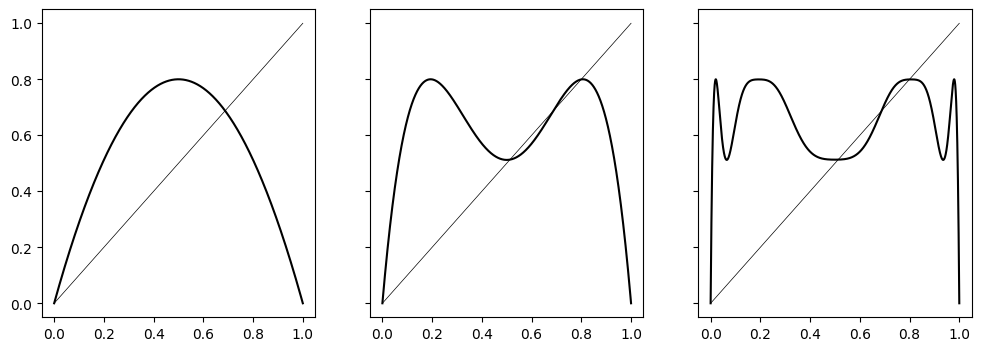
\includegraphics[scale=0.4]{images/h_3,2.png}
\caption{Gráficos de $h^2$ e $h^4$ para $\mu = 3.2$.}
\end{figure}
\end{block}

\end{columns}
\end{frame}

%--------------------

\begin{frame}
\vspace{5pt}
\frametitle{Teorema de Sharkovsky}
\begin{columns}
\column{\dimexpr\paperwidth-15pt}

Se, por exemplo, $\per_5(f) \neq \emptyset$ implica que $\per_3(f) \neq \emptyset$, então os números $3$ e $5$ podem trocar de lugar na ordenação de Sharkovsky. O seguinte teorema mostra que isso não é possível.

\begin{theorem}
Se $n \geq 1$, então existe uma função $f$ com as seguintes propriedades:
\begin{enumerate}
\item $\per_n(f) \neq \emptyset$.
\item $\per_m(f) =  \emptyset$ para todo $m \, \triangleright \, n$.
\end{enumerate}
\end{theorem}

\end{columns}
\end{frame}
